\appendix
\chapter{RADARの有用性の検証}
 ここではRADARとLiDARにおける環境依存性について検証を行う.

\section{検証手法}
\subsection{センサ}
 比較対象としてRADARと同じ価格帯のLiDARを用意した.使用したLiDARの性能と外観を表\ref{tab:lidar_spec_table},図\ref{fig:lidar}に示す.\cite{lidar_datasheet}

\begin{table}[htbp]
    \centering
    \caption{LiDARの性能}
    \begin{tabular}{|l|l|}
\hline
製品名   & YDLIDAR X4 \\ \hline
検出距離  & 120〜11,000mm \\ \hline
走査視野  & 360° \\ \hline
角分解能  & 0.5° \\ \hline
走査周波数 & 6〜12Hz \\ \hline
電源電圧  & DC5V \\ \hline
消費電流  & 450mA \\ \hline
\end{tabular}

    \label{tab:lidar_spec_table}
\end{table}

\begin{figure}[H]
    \centering
    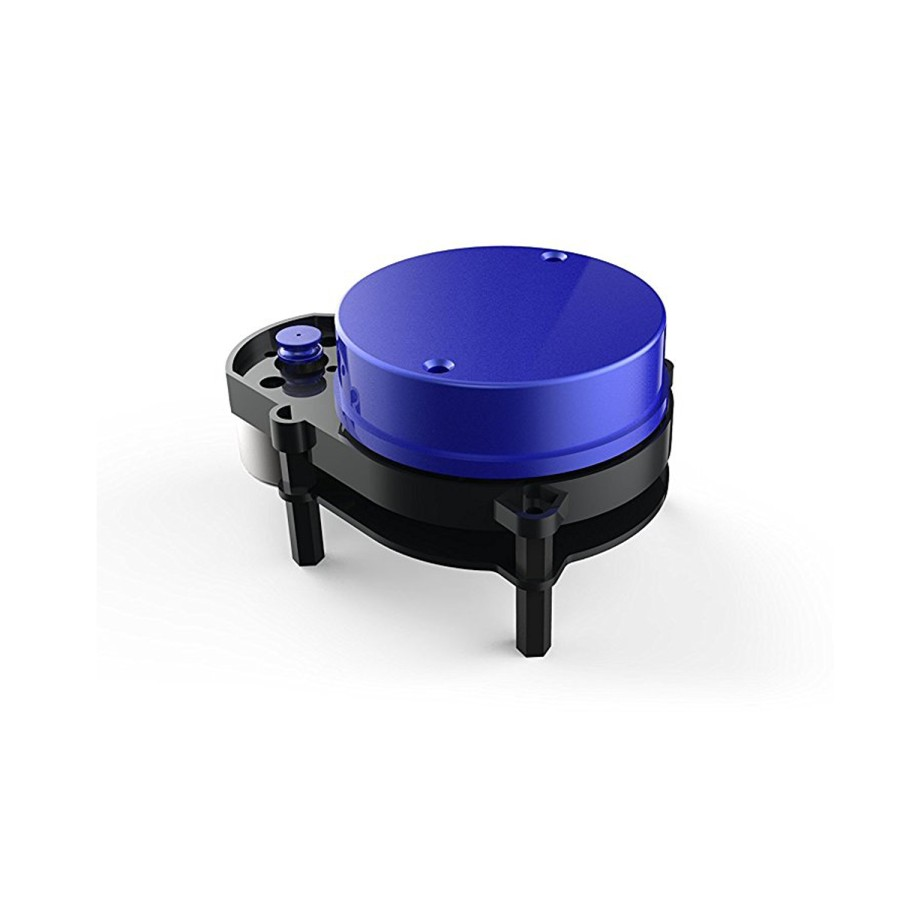
\includegraphics[width=8cm]{./fig/lidar.jpg}
    \caption{測定に使用したLiDAR}
    \label{fig:lidar}
\end{figure}
 なお,LiDARは仕様上,全方向(ヨー角360度)をスキャンするが,今回の実験では壁側の1本のレーザーだけ使用する.

\subsection{実験環境}
 壁との距離をセンサで24時間計測する.この際の実験環境を表\ref{tab:comp_env_table},実験の様子を図\ref{fig:comparison_measure_environment}に示す.

\begin{table}[htbp]
    \centering
    \caption{実験環境}
    \begin{tabular}{|l|r|}
    \hline
    測定日時  & 2020/01/12 08:47〜2020/01/12 08:47 \\ \hline
    測定場所  & 一関高専4号棟402号室 \\ \hline
    測定環境  & 無人,消灯,外からの外乱光あり \\ \hline
    対象物までの距離 & 0.6m \\ \hline
    測定間隔  & 10秒 \\ \hline
\end{tabular}
    \label{tab:comp_env_table}
\end{table}

\begin{figure}[H]
    \centering
    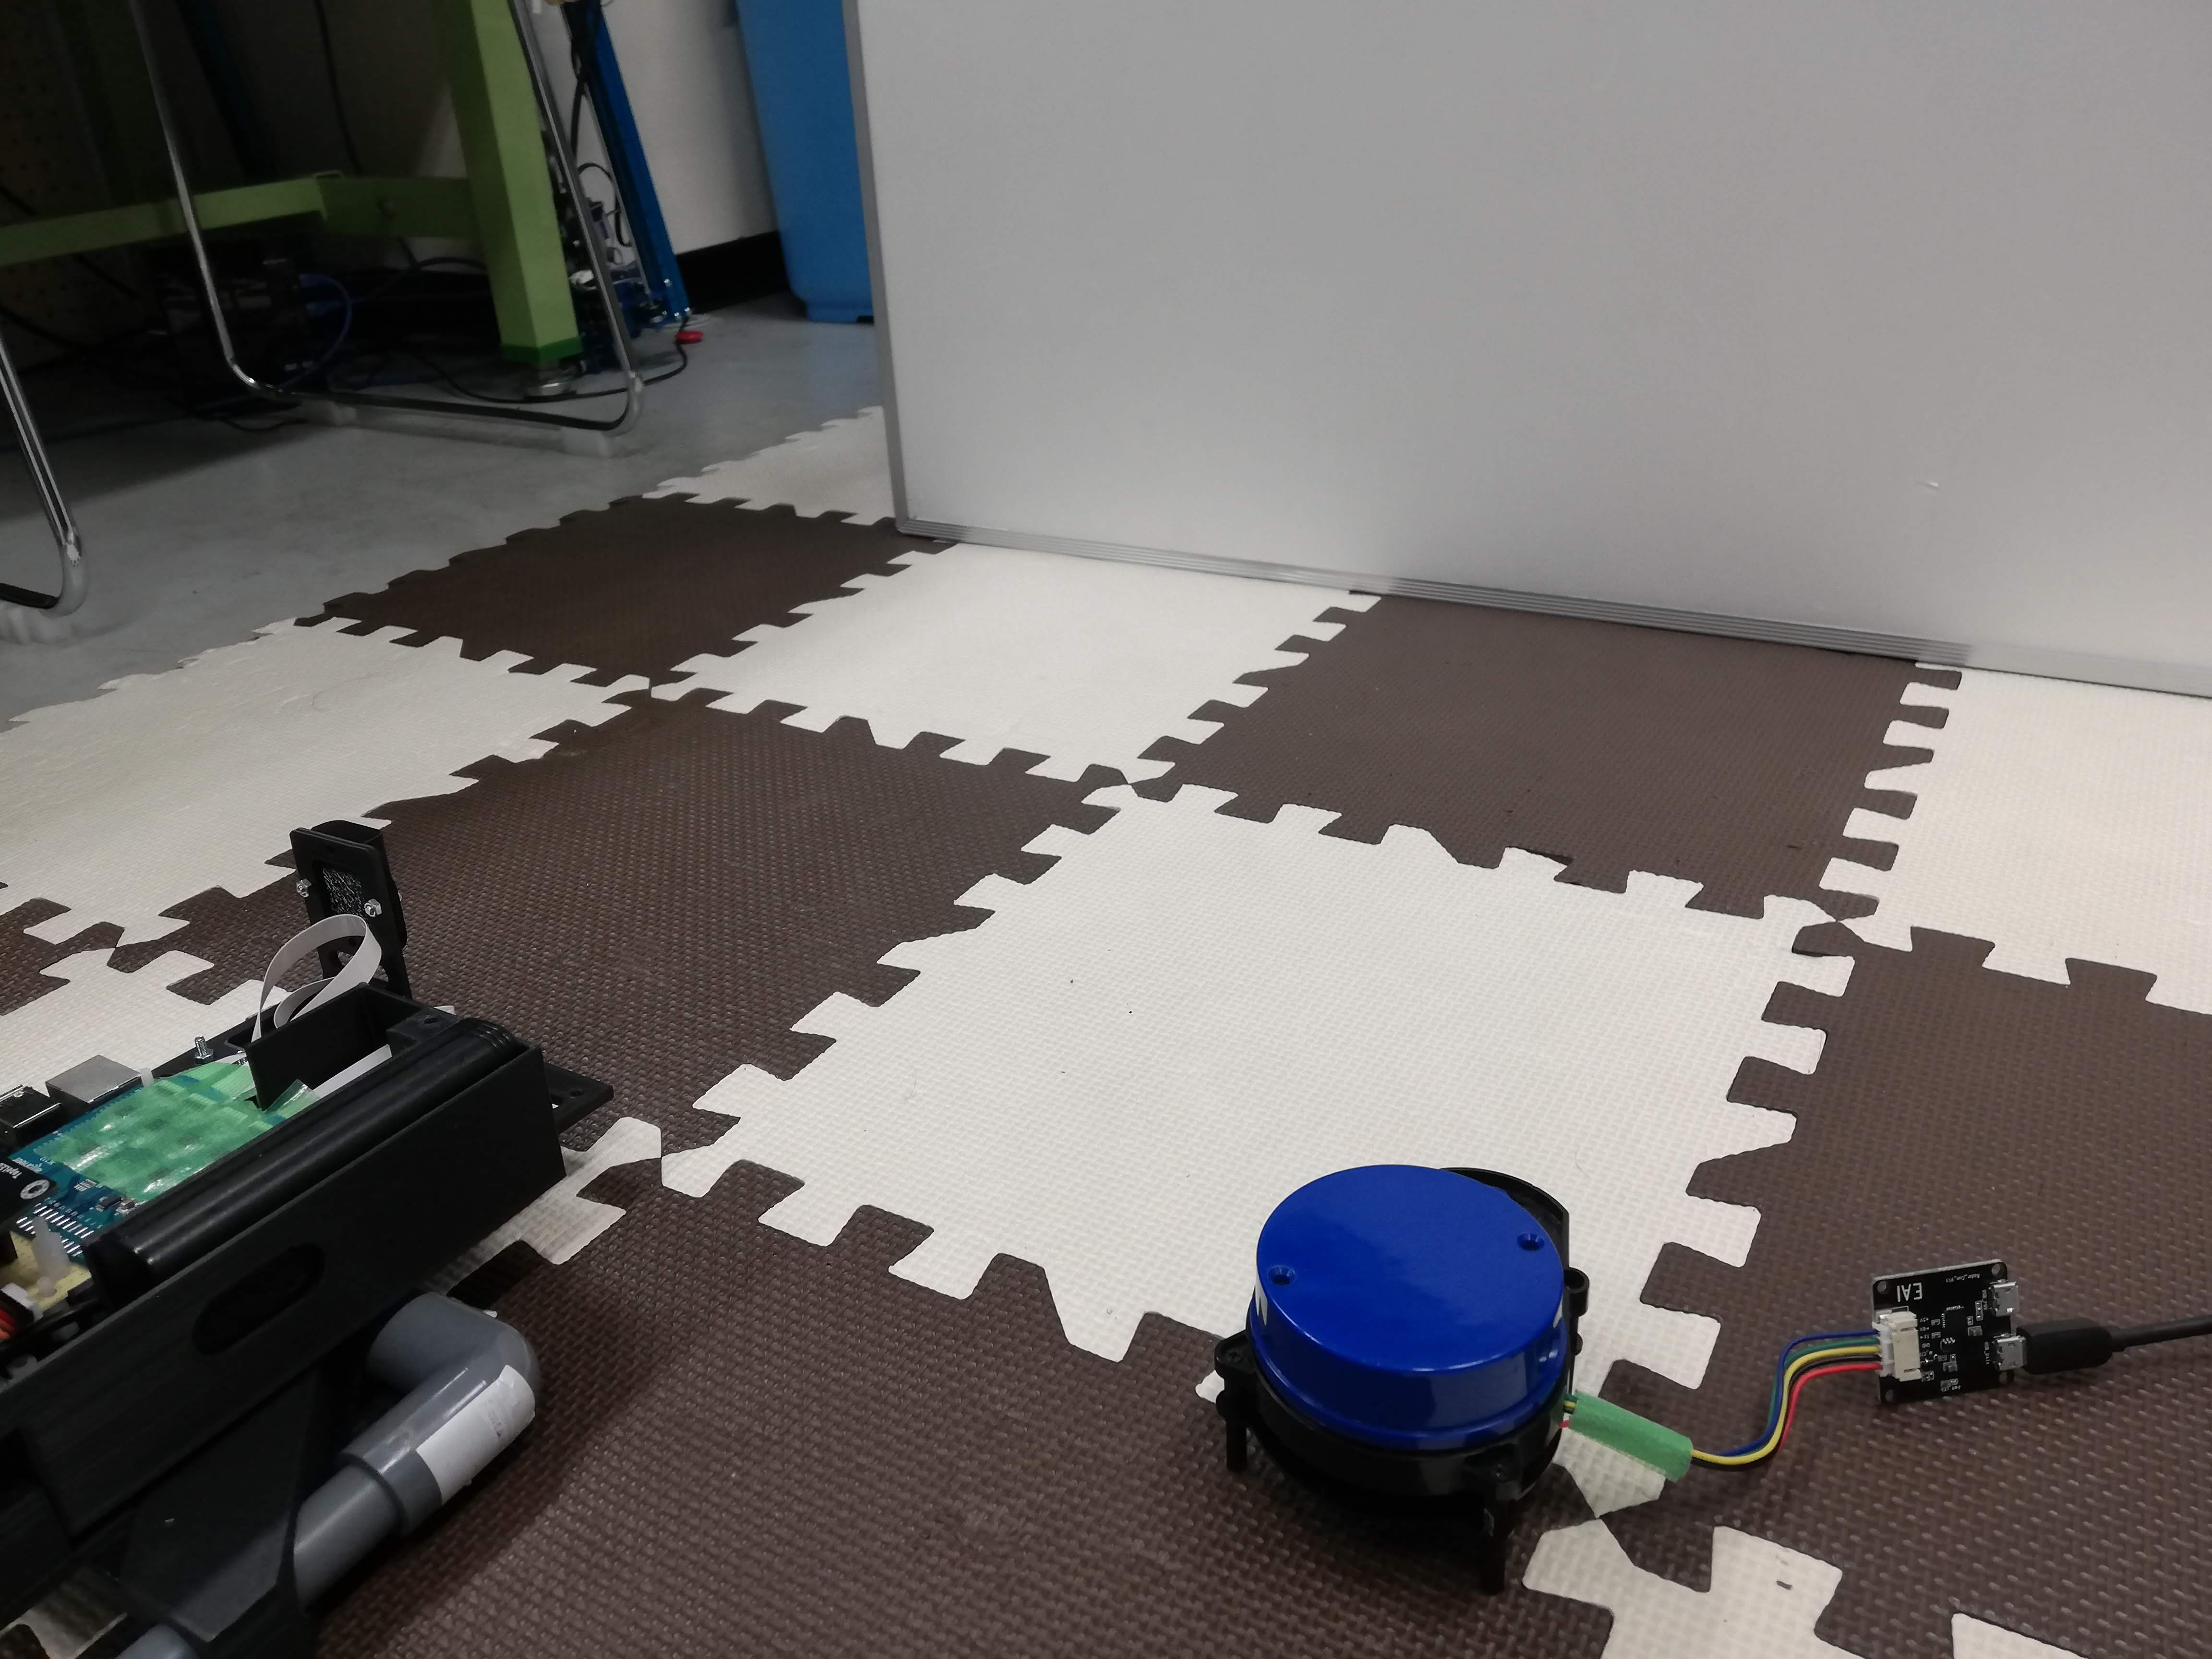
\includegraphics[width=8cm]{./fig/comparison_measure_environment.jpg}
    \caption{RADARとLiDARの比較実験の様子}
    \label{fig:comparison_measure_environment}
\end{figure}

\section{測定結果}
 RADAR,LiDARから得られた観測データを図\ref{fig:comparison_raw}に示す.また,センサの平均値,分散値を表\ref{tab:comp_result_table}にまとめる.
\begin{figure}[H]
    \centering
    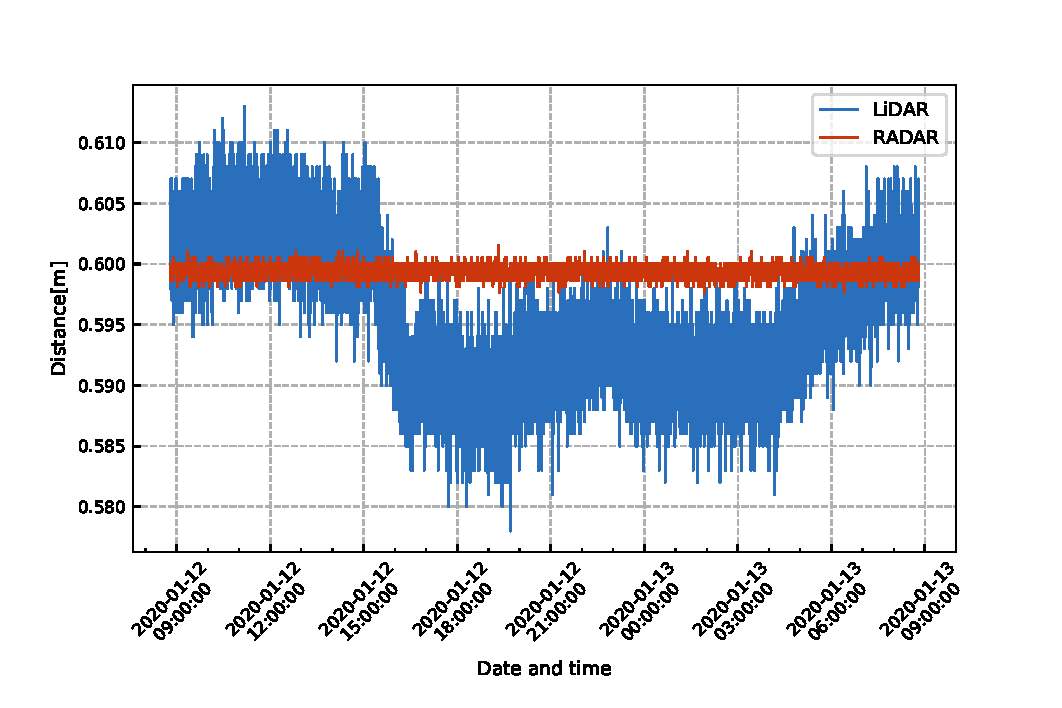
\includegraphics[width=11cm]{./fig/comparison_raw.pdf}
    \caption{LiDARとRADARの測定値の推移}
    \label{fig:comparison_raw}
\end{figure}

\begin{table}[htbp]
    \centering
    \caption{実験結果}
    \begin{tabular}{crr}
\hline
        & \multicolumn{1}{c}{LiDAR} & \multicolumn{1}{c}{RADAR} \\
\hline
\hline
平均    & 0.59538803 & 0.59935253 \\
\hline
中央値   & 0.59500000 & 0.59958800 \\
\hline
分散    & 0.00003424 & 0.00000024 \\
\hline
標準偏差  & 0.00585180 & 0.00049350 \\
\hline
\end{tabular}

    \label{tab:comp_result_table}
\end{table}


 図\ref{fig:comparison_raw}のデータに対して移動平均フィルタを施した.フィルタ処理後のデータを図\ref{fig:comparison_filtered60}に示す.
\begin{figure}[H]
    \centering
    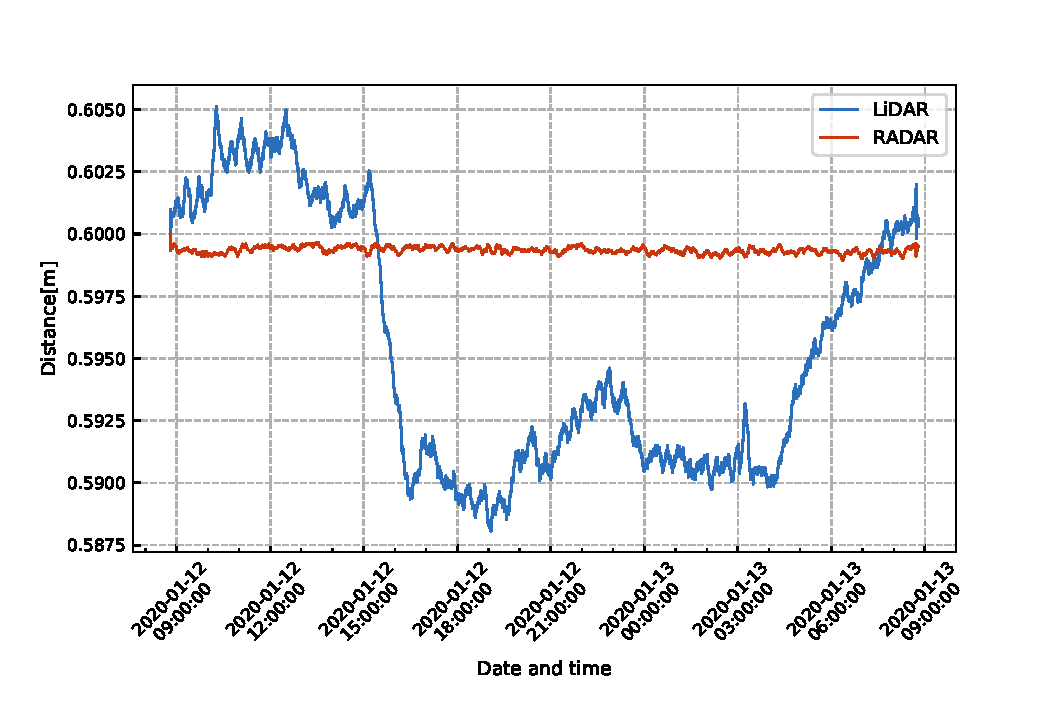
\includegraphics[width=11cm]{./fig/comparison_filtered60.pdf}
    \caption{LiDARとRADARの測定値の推移(移動平均フィルタ処理後)}
    \label{fig:comparison_filtered60}
\end{figure}

\section{結論}
 表\ref{tab:comp_result_table}からLiDARと比較してRADARの方が値のばらつきが小さいことがわかった.しかし,LiDARとRADARでは測定原理が異なるため,単純にこのデータだけでRADARの方が優れているとは言い切れない.そこで,図\ref{fig:comparison_filtered60}を見ると,LiDARは時間経過に対応して得られるデータが変動している.測定を行なった2020年1月12日の一関市の日没は16:33,1月13日の日の出は6:54であった.LiDARの測定値が大きく変動している時間と日没,日の出の時間はおおよそ一致していることから,この値の変動は外からの太陽光の影響を受けた可能性がある.また,測定を行なった部屋では温度,湿度の管理を行なっていなかったため,光以外の環境的要因によって測定値にばらつきが出た可能性も考えられる.\\
 一方でRADARは24時間を通してほぼ一定の値を取り続けていた.このことから,RADARはLiDARと比較して外乱の影響を受けにくいと考えられる.以上より,RADARは他の車載センサと比較して環境変化に対しての優位性があると結論づける.